\chapter{Comunicazione Multicast in IPv4}

\section{Introduzione al Multicast}

La comunicazione Multicast a livello IP nasce per risolvere in modo efficiente ed elegante un problema specifico: un singolo nodo sorgente deve inviare lo stesso flusso di dati a molteplici destinazioni simultaneamente. Esempi tipici di questo scenario, denominato \textit{group communication}, includono le videoconferenze e il \textit{video broadcasting} (come la trasmissione in diretta di un evento sportivo).

\subsection{Confronto con Broadcast e Unicast}
Per comprendere l'utilità del Multicast, è utile confrontarlo con le due alternative tradizionali:
\begin{itemize}
    \item \textbf{Broadcast:} Inviare il pacchetto a tutti i nodi della rete. A livello geografico (Internet), questa soluzione non è praticabile, in quanto inonderebbe la rete globale di pacchetti non richiesti. A livello IP, un vero broadcast su scala geografica non è infatti supportato.
    \item \textbf{Unicast:} La sorgente instaura una comunicazione punto-a-punto con ogni singola destinazione. Se mille utenti vogliono assistere all'evento in streaming, la sorgente deve aprire mille sessioni separate e inviare mille copie dello stesso pacchetto. Questa soluzione non scala, in quanto satura rapidamente la banda in uscita della sorgente e dei router a essa vicini.
\end{itemize}

\subsection{Principi di Funzionamento e Vantaggi}
La comunicazione Multicast si posiziona come una via di mezzo estremamente efficiente. L'idea fondamentale è che \textbf{la sorgente invia una sola copia del pacchetto}. Sarà poi l'infrastruttura di rete (ovvero i router) ad assumersi l'onere di duplicare il pacchetto, inoltrandolo su percorsi diversi \textit{soltanto} quando e dove è strettamente necessario (ossia dove è presente almeno un utente interessato).

% FIGURA ORIGINALE DA RECUPERARE DALLE SLIDE
% Slide di provenienza: 3 (sottointesa dall'inizio della spiegazione)
% Tipo: schema
% Descrizione: Schema che mostra un nodo sorgente che invia un singolo flusso e i router che duplicano i pacchetti solo verso i rami della rete in cui sono presenti host interessati.
% Punto di inserimento: dopo la spiegazione del concetto base di multicast.
% File da inserire: albero_multicast_routing

\begin{figure}[H]
    \centering
    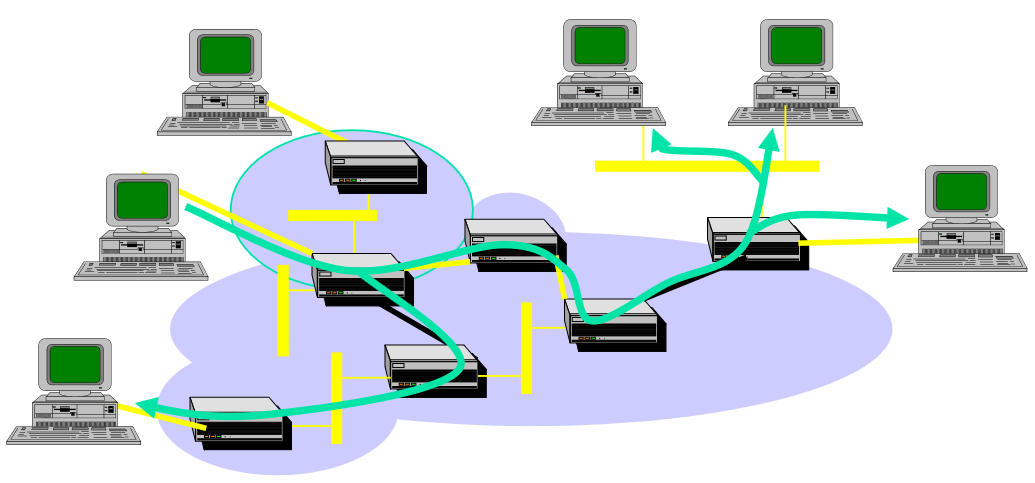
\includegraphics[width=0.85\textwidth]{capitoli/01f - IPv4Multicast/images/albero_multicast_routing}
    \caption{Principio di instradamento Multicast: la sorgente invia un singolo pacchetto, che viene duplicato dai router unicamente sui percorsi necessari per raggiungere le destinazioni.}
    \label{fig:multicast-tree}
\end{figure}

Un'altra caratteristica cruciale del Multicast è la sua forte \textbf{dinamicità}. Gli host non sono entità passive, ma scelgono attivamente di unirsi (\textit{join}) o abbandonare (\textit{leave}) un gruppo in qualsiasi momento. La sorgente non deve preoccuparsi di tenere traccia di chi si connette o si scollega: invia semplicemente il traffico verso un indirizzo logico di gruppo, disinteressandosi del numero e della posizione dei riceventi. Tutta la complessità gestionale è delegata alla rete.

\section{Indirizzamento Multicast a Livello IP}

Per fare in modo che un pacchetto venga interpretato come destinato a un gruppo e non a un singolo host, è stato necessario definire uno spazio di indirizzamento dedicato. 

\subsection{Le Classi di Indirizzi e la Classe D}
Storicamente, in IPv4, questa necessità è stata soddisfatta introducendo la \textbf{Classe D}. Tutti gli indirizzi appartenenti a questa classe sono facilmente riconoscibili dai router perché iniziano invariabilmente con i bit \texttt{1110}.
Tradotto in formato decimale, l'intervallo di indirizzi Multicast va da:
\[ 224.0.0.0 \quad \text{a} \quad 239.255.255.255 \]

Un indirizzo IP di questo tipo non identifica una macchina fisica, ma un \textbf{gruppo di host} (es. "tutti gli utenti interessati alla partita di pallavolo"). Qualunque pacchetto inviato a tale indirizzo verrà consegnato a tutti gli host che si sono iscritti al gruppo, in qualsiasi punto della rete si trovino, a patto che i router intermedi supportino il routing multicast.

\subsection{Indirizzi Riservati e Ambiti d'Uso}
All'interno dello spazio della Classe D, la IANA (Internet Assigned Numbers Authority) ha riservato alcuni blocchi (secondo la RFC 5771) per scopi specifici:

\begin{itemize}
    \item \textbf{\texttt{224.0.0.0/24} (Link-local control):} Questo blocco ha validità esclusivamente a livello locale (all'interno della singola LAN). I pacchetti con questi indirizzi destinazione hanno il campo \texttt{TTL = 1} a livello IP e \textbf{non vengono mai inoltrati dai router} al di fuori della sottorete. Alcuni esempi notevoli:
    \begin{itemize}
        \item \texttt{224.0.0.1}: Indirizza tutti gli host presenti nella sottorete.
        \item \texttt{224.0.0.2}: Indirizza tutti i router presenti nella sottorete.
        \item \texttt{224.0.0.22}: Utilizzato dal protocollo IGMPv3.
        \item \texttt{224.0.0.251}: Utilizzato per il protocollo mDNS (Multicast DNS).
    \end{itemize}
    \item \textbf{\texttt{232.0.0.0/8} (Source-specific multicast - RFC 4607):} Utilizzato in scenari in cui gli host non si iscrivono solo a un gruppo generico, ma richiedono esplicitamente di ricevere traffico per quel gruppo proveniente da una \textit{sorgente specifica}.
    \item \textbf{\texttt{239.0.0.0/8} (Administratively scoped - RFC 2365):} È l'equivalente degli indirizzi IP privati (come il \texttt{192.168.x.x}) per il Multicast. Può essere usato liberamente all'interno di una rete aziendale o privata senza rischiare conflitti su Internet.
\end{itemize}

\section{Gestione dei Gruppi a Livello Locale: IGMP}

Affinché la rete sappia dove recapitare i pacchetti, gli host devono comunicare il proprio interesse ai router locali. Questo avviene tramite il protocollo \textbf{IGMP (Internet Group Management Protocol)}.
\textit{Nota bene:} Non va confuso con ICMP (utilizzato da tool come \texttt{ping} o integrato in procedure come ARP). IGMP è specifico e dedicato esclusivamente alla gestione della "membership" dei gruppi Multicast. Viene incapsulato direttamente in datagrammi IPv4 e scambiato tra host e router a livello locale (con \texttt{TTL = 1}).

\begin{figure}[H]
    \centering
    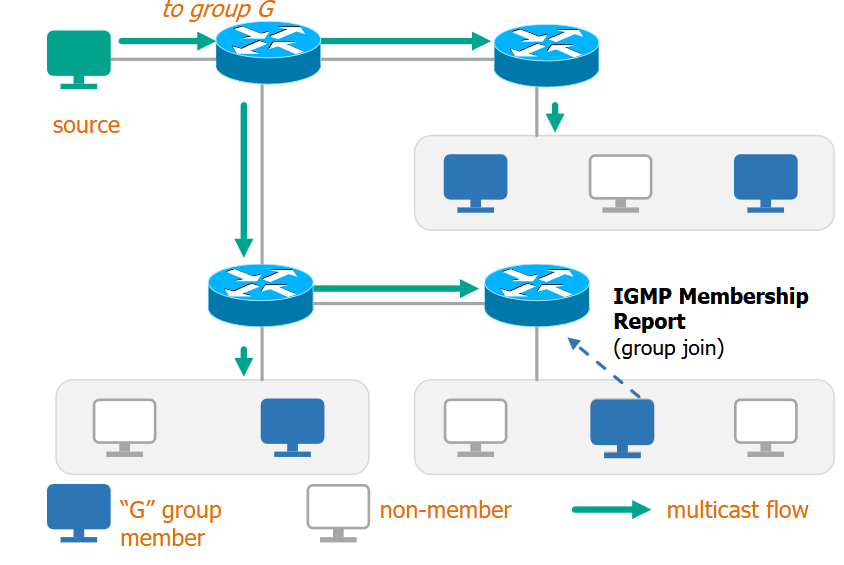
\includegraphics[width=0.85\textwidth]{capitoli/01f - IPv4Multicast/images/igmp-join-leave}
    \caption{Schema di funzionamento del protocollo IGMP: gli host inviano messaggi di join e leave ai router per iscriversi o abbandonare un gruppo Multicast.}
    \label{fig:igmp-join-leave}
\end{figure}

\subsection{Iscrizione e Abbandono di un Gruppo}
Quando un dispositivo o un'applicazione richiede l'accesso a un flusso Multicast (es. gruppo $G$), esegue una \textit{join}. L'host genera un messaggio IGMP chiamato \textbf{Membership Report} inviandolo all'indirizzo speciale dedicato ai router (\texttt{224.0.0.22}). 
Il router, ricevendo questo messaggio, comprende che all'interno di quella specifica LAN vi è almeno un host interessato a $G$. Da questo momento, il router si configurerà, dialogando con gli altri router della rete globale, per ricevere i pacchetti diretti a $G$ e iniettarli nella LAN.

Se un secondo host nella stessa LAN si iscrive al medesimo gruppo, manderà un altro Membership Report. Per il router non cambia operativamente nulla sul fronte geografico: sa già di dover inoltrare il traffico nella LAN, deve solo tenere traccia del fatto che ora gli host interessati sono molteplici.

Quando un host termina la visualizzazione (es. l'utente chiude il software di streaming), il protocollo prevede l'invio di un messaggio di \textit{leave}. Finché vi è almeno un altro host attivo, il router continua a instradare il traffico nella LAN. Quando l'ultimo host invia il messaggio di leave, il router cessa di richiedere i dati per il gruppo $G$ al resto della rete.

\subsection{Il Problema dell'Abbandono Silenzioso e le Query del Router}
Nella realtà operativa, gli host non inviano sempre in modo diligente il messaggio di leave. Un utente potrebbe chiudere bruscamente un'applicazione, spegnere il PC togliendo la corrente o perdere la connessione, uscendo dal gruppo senza informare il router.
Se il router si basasse unicamente sui messaggi di leave espliciti per interrompere il flusso, la rete finirebbe per essere intasata da flussi Multicast inoltrati in reti locali prive di ascoltatori reali.

Per risolvere questo problema, IGMP affida al router un ruolo proattivo: periodicamente (es. ogni 3, 5 o 10 minuti), il router invia messaggi di \textbf{IGMP General Query} nella LAN. In sostanza, il router chiede in multicast: \textit{"C'è ancora qualcuno interessato ai gruppi attivi?"}.
Se un host è ancora in ascolto, deve rispondere ri-confermando il proprio interesse con un Membership Report. Se, trascorso un certo \textit{timeout}, il router non riceve alcuna risposta per un determinato gruppo, assume che tutti gli host abbiano abbandonato e provvede a bloccare l'inoltro di quel traffico, ottimizzando l'uso della banda.

\section{Multicast a Livello di Collegamento (IEEE 802)}

Tutto ciò che abbiamo descritto avviene a livello di Rete (Livello 3). Tuttavia, nella trasmissione pratica dei dati, il datagramma IP deve essere incapsulato in una trama di livello Datalink (Livello 2), ad esempio Ethernet, che utilizza gli indirizzi MAC fisici a 48 bit. 
Sorge quindi un problema: se a livello IP l'indirizzo destinazione è un gruppo (es. \texttt{224.0.0.1}), cosa inseriamo come MAC destinazione? Non possiamo inserire il MAC specifico dell'host 2 o dell'host 3, poiché violerebbe il principio del Multicast (non sapendo a priori chi ascolta e impedendo agli altri di processare la trama).

\subsection{Mappatura degli Indirizzi da IPv4 a MAC}
Per risolvere la questione, l'RFC 7042 ha stabilito una procedura matematica fissa per derivare un "MAC Multicast" direttamente dall'indirizzo IP Multicast. Poiché dobbiamo passare da un identificativo a 32 bit (IP) a uno a 48 bit (MAC), e considerando che a livello IP l'identificativo effettivo del gruppo occupa 28 bit (tolti i 4 bit del prefisso della Classe D), si opera in questo modo:

\begin{enumerate}
    \item \textbf{I primi 25 bit del MAC sono fissati.} Si utilizza l'Organizationally Unique Identifier (OUI) \texttt{01-00-5E}, a cui si aggiunge un bit posto a \texttt{0}. 
    \item \textbf{Gli ultimi 23 bit del MAC} vengono banalmente copiati dagli ultimi 23 bit dell'indirizzo IP Multicast.
\end{enumerate}

% FIGURA ORIGINALE DA RECUPERARE DALLE SLIDE
% Slide di provenienza: 6
% Tipo: diagramma
% Descrizione: Diagramma che mostra la traduzione dei bit da un indirizzo IPv4 Multicast (Classe D) a un indirizzo MAC, evidenziando il prefisso 01-00-5E, il bit 0 fisso e i 23 bit copiati dall'IP.
% Punto di inserimento: dopo la spiegazione della procedura di mappatura.
% File da inserire: mapping_ip_mac_multicast

\begin{figure}[H]
    \centering
    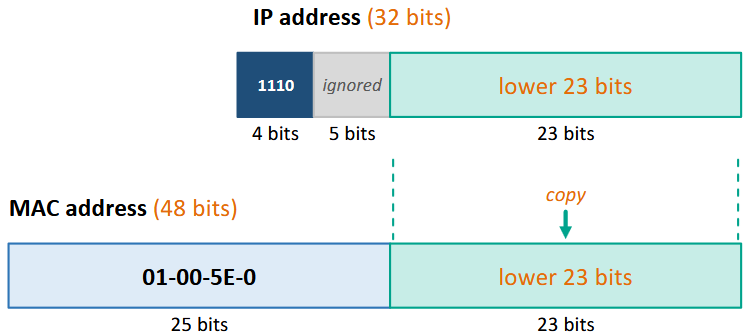
\includegraphics[width=0.6\textwidth]{capitoli/01f - IPv4Multicast/images/mapping_ip_mac_multicast}
    \caption{Costruzione di un indirizzo MAC Multicast a partire da un indirizzo IP di Classe D (RFC 7042).}
    \label{fig:mac-mapping}
\end{figure}

\subsubsection{Significato tecnico del byte iniziale e collisioni}
Come approfondimento a livello hardware, c'è un motivo per cui si usa proprio il byte iniziale \texttt{01} (in binario \texttt{00000001}). La tecnologia Ethernet trasmette in modalità \textit{Little Endian}, inviando per primo il bit meno significativo del byte. Di conseguenza, quel byte fa sì che il primo bit assoluto che viaggia sul cavo sia un \texttt{1}. A livello hardware, questo segnale immediato permette alle schede di rete in ascolto di capire all'istante che sta iniziando la ricezione di una trama Multicast.

Si noti inoltre che, copiando solo 23 dei 28 bit che identificano il gruppo a livello IP, ben 5 bit dell'IP vengono ignorati. Questo significa che più indirizzi IP Multicast differenti mapperanno esattamente sullo stesso indirizzo MAC Multicast. Le conseguenti "collisioni" a livello MAC non sono un errore fatale: la trama viene passata al livello di rete, e sarà il livello IP dell'host a verificare l'indirizzo destinazione reale, scartando il pacchetto se l'IP non corrisponde al gruppo richiesto.

\subsection{Comportamento delle Schede di Rete (NIC)}
A livello locale, per ricevere i pacchetti, il sistema operativo deve istruire la scheda di rete fisica (NIC - Network Interface Card) affinché non scarti le trame destinate al nuovo MAC Multicast calcolato. 
Poiché in una rete molto dinamica le iscrizioni e gli abbandoni ai gruppi possono essere frequentissimi, riprogrammare continuamente la configurazione hardware della NIC risulta inefficiente. Molto spesso, i costruttori configurano le NIC in una modalità "promiscua per il Multicast": la scheda hardware non scarta mai le trame che presentano il prefisso MAC Multicast (\texttt{01:00:5E}). Le accetta tutte e le inoltra al sistema operativo, lasciando al livello IP (software) il rapido compito di verificare e scartare i pacchetti dei gruppi a cui l'host non è attualmente iscritto.

\subsection{Gestione del Multicast negli Switch: IGMP Snooping vs Flooding}
Se la rete locale è composta da un singolo cavo coassiale (topologia a bus condiviso), ogni segnale elettrico raggiunge tutti gli host in modo nativo. Nelle reti moderne basate su Switch, la situazione è diversa. Lo switch, per sua natura, filtra il traffico a livello 2 inoltrando la trama solo sulla porta associata al MAC destinazione (comunicazione unicast). Ma nel caso di un MAC Multicast associato a un gruppo, come si comporta lo switch per far arrivare il pacchetto solo agli host realmente iscritti?
Esistono due approcci:

\begin{itemize}
    \item \textbf{IGMP Snooping:} Lo switch opera con un approccio \textit{cross-layer}. Invece di limitarsi a leggere l'header MAC (Livello 2), "sbircia" (snooping) nei messaggi IGMP a livello IP (Livello 3) per capire autonomamente su quali porte fisiche sono attestati gli host che hanno richiesto l'iscrizione al gruppo. Questo metodo è precisissimo e risparmia banda inviando i pacchetti solo agli host che li desiderano. Tuttavia, richiede switch intelligenti, capaci di operare a livello 3, aumentando la complessità e il costo dell'hardware.
    
    \begin{figure}[H]
        \centering
        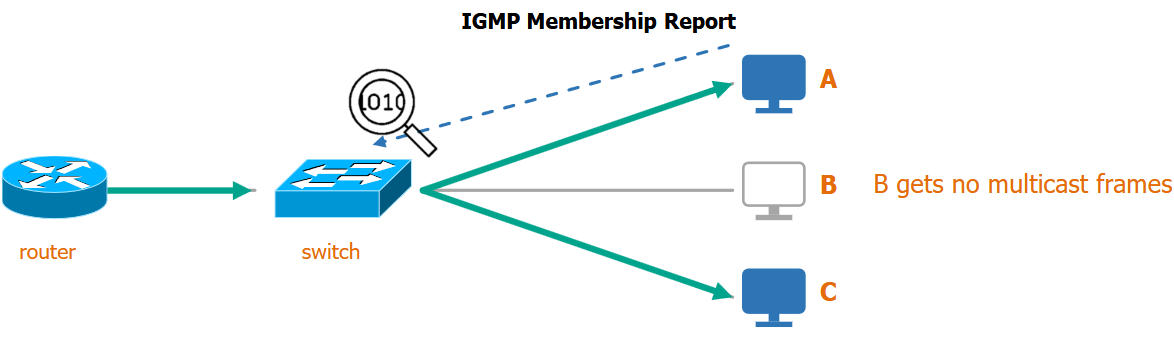
\includegraphics[width=0.7\textwidth]{capitoli/01f - IPv4Multicast/images/igmp-snooping}
        \caption{Schema di funzionamento dell'IGMP Snooping: lo switch "sbircia" i messaggi IGMP per costruire una mappa delle porte interessate a ciascun gruppo Multicast, inoltrando i pacchetti solo dove necessario.}  
    \end{figure}

    \item \textbf{Flooding:} È l'approccio largamente preferito per motivi di costo. Semplicemente, la funzionalità IGMP Snooping non viene abilitata, e lo switch viene istruito a trattare il traffico Multicast come fosse traffico Broadcast: se riceve una trama Multicast, la copia ciecamente e la inoltra (\textit{flooding}) su \textbf{tutte le porte} tranne quella da cui l'ha ricevuta. 
    Questa soluzione spreca una frazione di banda a livello locale, inviando trame a host non interessati (che poi le scarteranno tramite OS/NIC), ma permette di utilizzare switch economici, delegando i filtraggi ai terminali riceventi. Nelle moderne reti LAN, l'abbondanza di banda rende questo "spreco" del tutto accettabile.
\end{itemize}

\section{Multicast su Scala Geografica}

Uscendo dalla singola rete locale, si passa alla gestione globale tra reti connesse da molteplici router. 
Se il protocollo IGMP regola efficacemente la comunicazione tra l'host e il primo router della propria rete, non è sufficiente per mettere d'accordo router di operatori differenti che interconnettono reti separate, specialmente in presenza di collegamenti punto-a-punto (\textit{point-to-point}) privi di host intermedi in grado di generare messaggi IGMP.

\subsection{Protocolli di Routing Multicast}
Per operare su scala geografica, i router necessitano di \textbf{Multicast Routing Protocols} dedicati. 
Proprio come i protocolli di routing classici costruiscono in automatico le tabelle di instradamento scambiandosi informazioni per le reti Unicast, esistono protocolli specifici o estensioni in grado di far dialogare i router affinché si informino a vicenda sulla presenza di host interessati a specifici indirizzi IP Classe D.

L'obiettivo di questi protocolli è costruire, per ciascun gruppo host attivo, un \textit{distribution tree} (albero di distribuzione). L'albero parte dalla sorgente e si ramifica raggiungendo unicamente le LAN che possiedono almeno un utente membro del gruppo, garantendo che i router interrotti da connessioni punto-a-punto ricevano la direttiva di inoltro corretta.

\section{Esempi Applicativi e Stato di Adozione}

\subsection{Multicast DNS (mDNS) per la Scoperta dei Servizi}
Un caso di successo straordinario del Multicast a \textbf{livello locale} è la risoluzione dei nomi e la scoperta dei dispositivi sulla rete senza l'ausilio di un server DNS centrale (RFC 6762). 
Questa tecnologia, nota come \textbf{mDNS}, utilizza l'indirizzo Multicast \texttt{224.0.0.251}.

In una rete domestica o d'ufficio, quando si cerca una stampante, una Apple TV, un dispositivo Chromecast o un sistema AirPlay, il proprio dispositivo (tramite tecnologie come Apple Bonjour o Avahi su Linux/Windows) invia una query DNS verso il gruppo Multicast \texttt{224.0.0.251}. 
Ad esempio, invia il messaggio: \textit{"Ci sono ricevitori AirPlay in ascolto?"}. I dispositivi che offrono il servizio, in ascolto su quell'indirizzo, rispondono al gruppo. I nomi assegnati terminano tipicamente in \texttt{.local}.

Poiché questi indirizzi rientrano nel range link-local (\texttt{224.0.0.0/24}), i router non li inoltrano mai all'esterno. La scoperta dei servizi rimane perciò opportunamente confinata all'interno della sottorete. In contesti molto grandi, come le reti Wi-Fi universitarie, il traffico mDNS generato da migliaia di dispositivi diviene eccessivo, costringendo gli amministratori di rete a filtrarlo o gestirlo tramite dei proxy.

\begin{figure}[H]
    \centering
    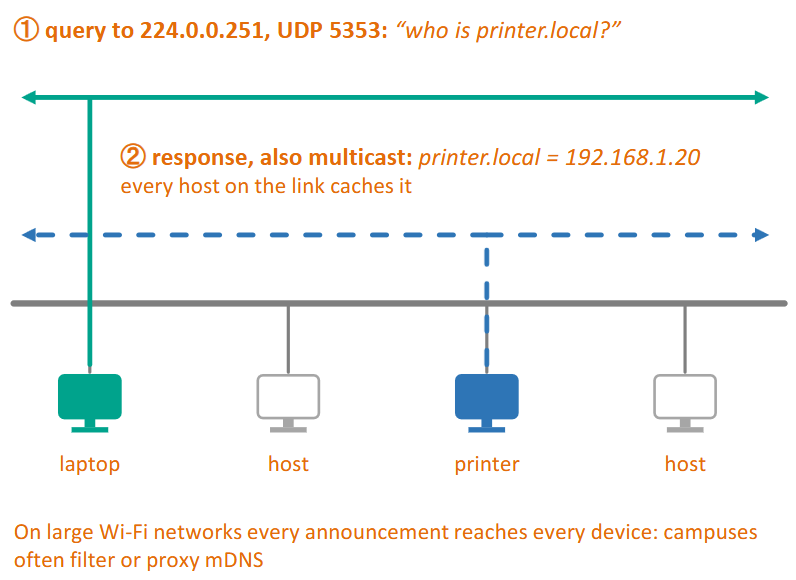
\includegraphics[width=0.6\textwidth]{capitoli/01f - IPv4Multicast/images/mdns}
    \caption{Esempio di funzionamento del protocollo mDNS: un host invia una query Multicast per scoprire i servizi disponibili, e i dispositivi che offrono tali servizi rispondono al gruppo.}
    \label{fig:mdns}
\end{figure}

\subsection{Limiti del Multicast e Scarsa Adozione su Scala Globale}
Se da un punto di vista teorico l'efficienza nel risparmio di risorse è indiscutibile, dal punto di vista operativo l'adozione del Multicast su vasta scala in Internet (traffico \textit{inter-domain}) è praticamente nulla. 
Il Multicast viene utilizzato estensivamente solo in ambienti controllati, come data center aziendali, all'interno del dominio di un singolo Internet Service Provider (ISP) per servizi televisivi proprietari, o nelle singole LAN (come descritto per mDNS).

Le motivazioni di questo fallimento globale sono principalmente tre:
\begin{enumerate}
    \item \textbf{Perdita di Controllo per gli Operatori (Traffic Engineering):} Gli ISP ottimizzano le reti dimensionandole in base a stime prevedibili. Con il Multicast, prevedere quanto traffico scorrerà e dove verrà duplicato diventa arduo, sottraendo all'operatore la capacità di operare in modo efficace con pratiche di Traffic Control.
    \item \textbf{Complessità Inter-domain:} Su Internet, il traffico attraversa reti gestite da ISP differenti. Coordinare protocolli di routing Multicast tra enti commerciali concorrenti, scambiandosi costantemente lo stato dei gruppi di utenti in ascolto, presenta innumerevoli ostacoli politici, commerciali e di configurazione.
    \item \textbf{Incompatibilità strutturale con il Protocollo TCP.} Questo è il motivo tecnico fondamentale, spiegato nel prossimo paragrafo.
\end{enumerate}

\subsection{Incompatibilità con il Protocollo TCP}
A livello applicativo, i servizi che muovono enormi volumi di dati video (come Netflix o YouTube) offrono agli utenti una qualità di servizio garantita. Per assicurare tale affidabilità e gestire dinamicamente aspetti come i pacchetti persi o la congestione della rete, questi colossi dello streaming si affidano saldamente al protocollo di trasporto \textbf{TCP (Transmission Control Protocol)}.

Il problema risiede nel fatto che il \textbf{TCP è un protocollo orientato alla connessione (\textit{connection-oriented})}. Per operare, TCP richiede preventivamente l'instaurazione formale di un canale logico stabile e uno scambio di stato esclusivo (una sessione) tra \textit{una} sorgente definita e \textit{una} singola destinazione.
Il paradigma Multicast è l'esatto opposto: un nodo invia "al buio" verso una rete, disinteressandosi totalmente di chi e quanti siano i riceventi. Non essendovi una singola destinazione univoca, \textbf{è concettualmente impossibile instaurare una sessione TCP su un canale Multicast}.

Perciò, il traffico Multicast deve operare esclusivamente appoggiandosi su protocolli \textit{connectionless} come l'\textbf{UDP (User Datagram Protocol)}. Poiché i fornitori commerciali prediligono il controllo sulla qualità offerto dal TCP, rinunciano volontariamente all'efficienza architetturale del Multicast, servendo gli utenti finali tramite un gran numero di flussi Unicast TCP. L'UDP (e conseguentemente il Multicast potenziale) resta relegato ad ambiti \textit{real-time} specifici, come porzioni di traffico per i videogiochi online, dove la velocità prevale sulla perdita di singoli pacchetti.